The framework of GSACO-O algorithm is illustrated in Figure~\ref{fig:aco-flowchart} and the input and internal parameters, 
is summarized in Table~\ref{tab:parameters}. 
The four main submodules, highlighted in bold, are discussed in detail in the following subsections.

\begin{figure}[t]
	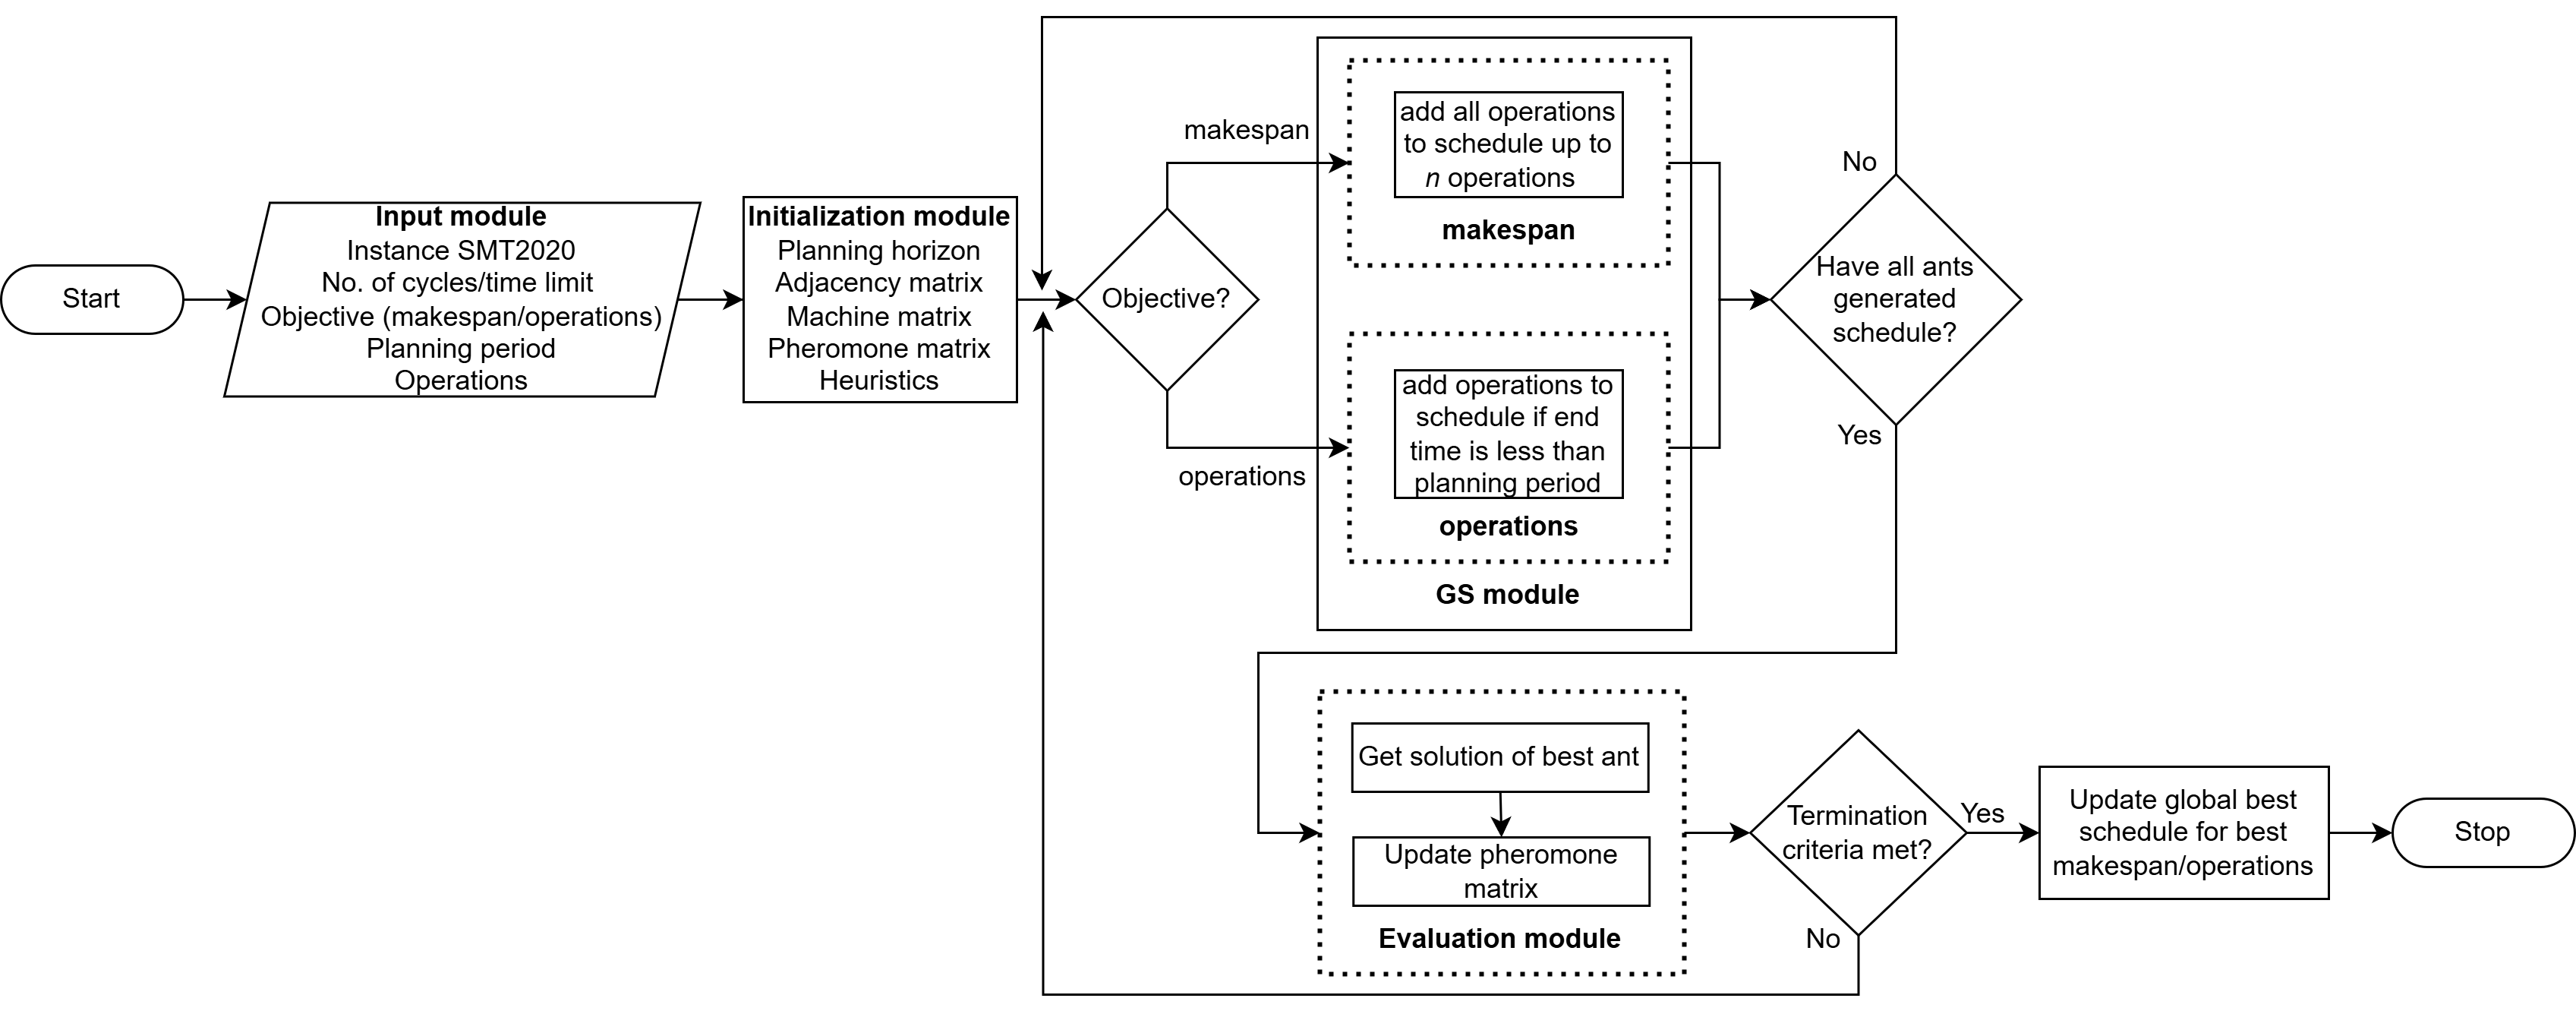
\includegraphics[width=\textwidth]{aco-flowchart.png}
	\caption{GSACO-O framework}
	\label{fig:aco-flowchart}
\end{figure}

\begin{table}[t]
	\caption{GSACO-O parameters}\label{tab:parameters} \centering
	\begin{tabular}{|l|l|}
		\hline
		Parameter & Description \\ \hline
		$o$ & Objective \\
		$l$ & Cycles/time limit        \\
		$n$ & Operations per lot \\
		$h$ & Planning horizon \\
		$k$ & Number of ants \\
		$\tau_{y}$ & Initial pheromone level \\
		$\tau_{z}$ & Minimum pheromone level \\
		$\tau_{e}$ & Pheromone level on edge $e$ \\
		%	$\eta_{e}$ & Heuristic information on edge $e$ \\
		$\rho$ & Evaporation rate \\
		$c$ & Contribution of best schedules \\
		%	$\alpha$ & Influence of pheromone $\tau_{e}$ \\
		%	$\beta$ & Influence of heuristic $\eta_{e}$    \\
		\hline
	\end{tabular}
\end{table}

For a configurable cycle number or time limit~$l$,
each of the $k$ ants applies greedy search
using the GS procedure with respect to the objective.
That is, the first GS phase constructs an operation sequence, which is
then taken as basis for greedily assigning the operations to machines
in the second phase.   
Note that the ants run independently, so that their GS trials
can be performed in parallel.
As a result, $k$ schedules along with edges between operations
(described in Subsection~\ref{subsec:initialization})
that have been selected for their construction are obtained.
If some of these schedules improves the makespan over the best
schedule found in previous iterations (if any),
the best schedule gets updated.
As common for ACO algorithms,
pheromones $\tau_e$ on edges~$e$ are subject to evaporation,
according to the formula $\rho\cdot\tau_e$,
while edges selected to construct the best schedule obtained
so far also receive a pheromone contribution,
calculated as $\tau_e+c$.
Such pheromone deposition increases the chance for edges contributing to the
current best schedule
to get re-selected % by the GS procedure
in forthcoming iterations.

Algorithm~\ref{gsaco} provides a pseudo-code representation of
GSACO-O for minimizing makespan and optimizing operations within the planning horizon.

\begin{algorithm}[t]
	\caption{Greedy Search-based ACO variant (GSACO-O) for scheduling}
	\label{gsaco}
	\KwIn{dataset, instance, $l$}
	\KwOut{best schedule found by ants}
	\KwParam{$o$, $n$, $h$, $k$, $\tau_{y}$, $\tau_{z}$, $\rho$, $c$}
	Initialize adjacency, pheromone, and machine matrix\; 
	\eIf{\text{o} == \text{Makespan}}{
		$\mathit{makespan}\leftarrow \infty$\;
	}{
		$\mathit{operations}\leftarrow 0$\;
	}
	\While{cycle or time limit $l$ is not reached}{
		\ForEach{ant \KwFrom $1$ \KwTo $k$}{
			Run GS procedure to find a schedule\;
		}
		\eIf{\text{o} == \text{Makespan}}{
			$\mathit{new}\leftarrow$ shortest makespan of ants' schedules\;
			\If{$\mathit{new}<\mathit{makespan}$}{
				$\mathit{makespan}\leftarrow \mathit{new}$\;
				$\mathit{best}\leftarrow$ an ant's schedule of minimum $\mathit{makespan}$\;
			}
		}{
			$\mathit{new}\leftarrow$ maximum operations of ants'\;
			\If{$\mathit{new}>\mathit{operations}$}{
				$\mathit{operations}\leftarrow \mathit{new}$\;
				$\mathit{best}\leftarrow$ an ant's schedule of maximum $\mathit{operations}$\;
			}
		}
		\ForEach{edge $e$ in pheromone matrix}{
			$\tau_{e} \leftarrow \max\{\rho\cdot\tau_e,\tau_z\}$\tcp*[r]{evaporation}
		}
		\ForEach{edge $e$ selected by $\mathit{best}$ ant}{
			$\tau_{e} \leftarrow \tau_e+c$\tcp*[r]{deposit pheromones}
		}
	}
	\Return $\mathit{best}$\;
\end{algorithm}


\subsection{Input Module}
This module reads in an SMSP instance obtained from SMT2020 dataset \cite{kopp2020smt2020}. Additionally, it also configures the instance from the simulator develop by \cite{Kovacs2022} for the average processing times of the operations. 
The instance includes tool groups with their respective machines, jobs currently in progress, and production routes. In terms of dynamic state, the processing times for these routes are stochastic. Conversely, the simulator provides observed averages for processing times and job releases. Additionally, the module takes several inputs for the GSACO-O optimization process such as the objective~$o$, planning period~$h$, 
operation per lot~$n$ and a limit~$l$ on either the number of cycles or the time allocated for optimization.

\subsection{Initialization Module}
\label{subsec:initialization}
In view of long production routes with hundreds of operations
in the SMT2020 dataset, we introduce a configurable operations per lot~$n$
as upper bound on the length $n_j$ of the operation sequence for a job~$j$.
The operations per lot thus constitutes a scaling factor for the size and
the resulting complexity of SMSP instances.
% This horizon is crucial in planning and decision-making, especially within large-scale production systems.
In practice, unpredictable stochastic events make long-term schedules obsolete and necessitate frequent re-scheduling,
where limiting $n$ upfront provides a means to
control the search and enable short response times.

To express SMSP as a search problem on graphs,
we identify an instance with the disjunctive graph

whose vertices~$V$ contain the operations $O_{i,j,t}$ plus
a dummy start node~$0$,
conjunctive edges\linebreak[1]%
%
\begin{equation}
	\begin{array}{@{}r@{}l@{}}
		E_c = {}
		& \{(0,O_{1,j,t_1}) \mid O_{1,j,t_1}\in V\}
		\\ {} \cup {}
		& \{(O_{i-1,j,t_{i-1}},O_{i,j,t_i}) \mid O_{i,j,t_i}\in V, i > 1\}
	\end{array}
\end{equation}
%
connect the dummy start node~$0$ to the first operation
and each operation on to its successor (if any) in the sequence for a job,
and disjunctive edges\linebreak[1]%
%
\begin{equation}
	E_d = \{(O_{i,j,t},O_{i',j',t}) \mid O_{i,j,t}\in V,O_{i',j',t}\in V, j\neq j'\}
\end{equation}
%
link operations (of distinct jobs) sharing a common tool group,
as such operations may be allocated to the same machine.

Any feasible schedule induces an acyclic subgraph $(V,E)$ of 
the disjunctive graph~$G$
such that $E_c\subseteq E$, and $(O_{i,j,t},O_{i',j',t})\in E_d\cap E$
iff $s_{i,j,t,m}+d_{i,j,t} < s_{i',j',t,m}$ for distinct jobs $j\neq j'$,
i.e., the operation
$O_{i,j,t}$ is processed before $O_{i',j',t}$ by the same machine~$m$
of tool group $t_m=t$.
Conversely,
the search for a high-quality solution can be accomplished by
determining an acyclic subgraph $(V,E)$ of~$G$ that represents a schedule
of short makespan.

For example, Table~\ref{tab:instance} shows a small instance that follows the explanation of the proposed GSACO-O algorithm.
In Table~\ref{tab:operations}, the operations belonging to two jobs can
be obtained with the parameter $n=5$. The average duration of the operations for given tool group is given in seconds to avoid float calculation. Later the duration is converted to the minutes for visualization purpose.  
The lots that belong to the products are shown in Table~\ref{tab:lots}. The lots are at different stages of the production identified by the step number.


\begin{table}[ht]
	\caption{Example instance}\label{tab:instance} 
	\begin{subtable}{0.5\textwidth}
		\caption{Operations}\label{tab:operations} 
		\centering
		\begin{tabular}{|l|l|l|l|}
			\hline
			No. & Operation & Tool group name & Avg duration (sec) \\ \hline
			$1$ & $O_{1,1,2}$ & TF\_Met\_FE\_45 & $588$ \\
			$2$ & $O_{2,1,3}$ & WE\_FE\_108 & $59$ \\
			$3$ & $O_{3,1,4}$ & WE\_FE\_83 & $62$ \\
			$4$ & $O_{4,1,5}$ & WE\_FE\_84 & $54$ \\
			$5$ & $O_{5,1,1}$ & LithoTrack\_FE\_115 & $130$ \\
			$6$ & $O_{1,2,2}$ & TF\_Met\_FE\_45 & $588$ \\
			$7$ & $O_{2,2,3}$ & WE\_FE\_108 & $59$ \\
			$8$ & $O_{3,2,4}$ & WE\_FE\_83 & $62$ \\
			$9$ & $O_{4,2,5}$ & WE\_FE\_84 & $54$ \\
			$10$ & $O_{5,2,0}$ & Litho\_FE\_111 & $130$ \\
			\hline
		\end{tabular}
	\end{subtable}%
	\begin{subtable}{0.5\textwidth}
		\caption{Lots}\label{tab:lots}
		\centering
		\begin{tabular}{|l|l|l|}
			\hline
			Lot & Product & Step \\ \hline
			$1$ & $1$ & $1$ \\
			$2$ & $2$ & $2$ \\
			$3$ & $1$ & $1$ \\
			$4$ & $2$ & $3$ \\
			$5$ & $1$ & $1$ \\
			$6$ & $2$ & $2$ \\
			$7$ & $1$ & $1$ \\
			$8$ & $2$ & $3$ \\
			$9$ & $1$ & $1$ \\
			$10$ & $2$ & $2$ \\
			\hline
		\end{tabular}
	\end{subtable}
\end{table}

Conjunctive edges connect the dummy start node~$0$ to
the operations which come first in their jobs and all operations to their successors.
In addition, mutual disjunctive edges link operations
to be processed on the same tool group.
Since the products are at different stages and the remaining operations to schedule are obtained from the step given in Table~\ref{tab:lots} up to the maximum step in Table~\ref{tab:operations} for corresponding lot and product. 
The resulting $(N+1)\times(N+1)$ adjacency matrix, where $N=43$ is the
total number of operations, $0$ entries indicate the absence, and
$1$ entries the existence of edges, is given in Figure~\ref{fig:a}.

\begin{figure}[h]
	\centering
	\begin{subfigure}{.45\columnwidth}
		\centering
		$\begin{array}{c@{}c}
			& \begin{array}{cccccccccc} 0 & 1 & 2 & \dots & 41 & 42 & 43 \end{array} \\
			\begin{array}{c} 0 \\ 1 \\ 2 \\ \vdots \\ 41 \\ 42 \\ 43 \end{array} &
			\left[\begin{array}{ccccccccc}
				0 & 1 & 0 & \dots & 0 & 0 & 1 \\ 
				0 & 0 & 1 & \dots & 0 & 0 & 0 \\ 
				0 & 0 & 0 & \dots & 1 & 0 & 0 \\ 
				\vdots & \vdots & \vdots & \ddots & \vdots & \vdots & \vdots \\
				0 & 0 & 0 & \dots & 0 & 1 & 0 \\ 
				0 & 0 & 0 & \dots & 0 & 0 & 1 \\ 
				0 & 0 & 1 & \dots & 0 & 0 & 0 \\
			\end{array}\right]
		\end{array}$
		\caption{Adjacency matrix}
		\label{fig:a}
	\end{subfigure}\hfill
	\begin{subfigure}{.45\columnwidth}
		\centering
		$\begin{array}{c@{}c}
			& \begin{array}{cccccccccccc} 1 & 2 & 3 & \dots & 10 & 11 & 12 \end{array} \\
			\begin{array}{c} 0 \\ 1 \\ 2 \\ \vdots \\ 41 \\ 42 \\ 43 \end{array} &
			\left[\begin{array}{cccccccccccc}
				0 & 1 & 0 & \dots & 0 & 0 & 0 \\ 
				0 & 0 & 1 & \dots & 0 & 0 & 0 \\ 
				0 & 0 & 0 & \dots & 1 & 0 & 0 \\ 
				\vdots & \vdots & \vdots & \ddots & \vdots & \vdots & \vdots \\
				0 & 0 & 0 & \dots & 0 & 1 & 0 \\ 
				0 & 0 & 0 & \dots & 0 & 0 & 1 \\ 
				0 & 0 & 1 & \dots & 0 & 0 & 0 \\
			\end{array}\right]
		\end{array}$
		\caption{Machine matrix}
		\label{fig:b}
	\end{subfigure}
	\caption{Matrices for instance in Table~\ref{tab:instance}} \centering
\end{figure}

As initial pheromone level on edges $e\in E_c\cup E_d$,
we take $\tau_y=1$ by default.
In general, representing pheromone levels by an $(N+1)\times(N+1)$
matrix similar to the adjacency matrix,
the entries~$\tau_{e}$ are initialized according to the following condition:\linebreak[1]%

\begin{equation}
	\tau_{e} =
	\begin{cases}
		\tau_y & \text{if $e\in E_c\cup E_d$} \\
		0      & \text{otherwise}
	\end{cases}
\end{equation} 

With $\tau_y=1$, this reproduces the adjacency matrix in Figure~\ref{fig:a}
as initial pheromone matrix for our example.

We additionally represent the possible machine assignments
by an $(N+1)\times M$ machine matrix, where $M$ is the total number of
machines.
For example, with two machines per tool group and the mapping
$t_m=\lceil \frac{m}{2} \rceil$ from machine identifiers
$m\in \{1,\dots,12\}$ to the tool groups $t\in\{1,\dots,6\}$,
responsible for processing the remaining operations in Table~\ref{tab:instance},
we obtain the machine matrix shown in Figure~\ref{fig:b}.

\subsection{GS Module}

The general goal of greedy search methods consists of using heuristic decisions
to find high-quality, but not necessarily optimal solutions in short time.
Within GSACO-O, each ant applies greedy search to efficiently construct some
feasible schedule for a given SMSP instance.
The GS procedure based on the given objective $o$, outlined by the pseudo-code in Algorithm~\ref{gs},
includes two phases: 
operation sequencing and machine assignment.
%

\begin{algorithm}[t]
	\caption{Greedy Search (GS)}
	\label{gs}
	\KwIn{horizon $h$}
	\KwOut{schedule, selected edges of an ant, and operations finished in horizon $h$}
	$\mathit{sequence}\leftarrow[]$\;
	$\mathit{selected}\leftarrow\emptyset$\;
	$\mathit{next}\leftarrow\{(0,O_{1,j,t}) \mid j\in\{1,\dots,J\}\}$\;
	%	\lForEach{$m\in\{1,\dots,M\}$}{$f_m\leftarrow 0$}
	\While{$\mathit{next}\neq\emptyset$}{
		%	$\mathit{\tau}=\sum_{e\in\mathit{next}}\tau_e$\;
		\lForEach{$e\in\mathit{next}$}{%}
		$p_e\leftarrow \frac{\tau_e}{\sum_{e'\in\mathit{next}}\tau_{e'}}$}
	Randomly select an edge $e$ based on $p_e$\;
	\For{selected edge $e=(O',O_{i,j,t})$}{
		$\mathit{sequence}.\mathrm{enqueue}(O_{i,j,t})$\;
		$\mathit{selected}\leftarrow\mathit{selected}\cup\{e\}$\;
		$\mathit{next}\leftarrow\{(O_1,O_2)\in\mathit{next} \mid O_2\neq O_{i,j,t}\}$\;
		$\begin{array}[b]{@{}r@{}l@{}}
			E \leftarrow {} &		
			\{(O_{i,j,t},O_{{i+1},j,t'}) \mid i<n_j\}
			%	  \cup {}
			\\ {} \cup {} &
			\{(O_{i,j,t},O_{i',j',t}) \mid (O_1,O_{i',j',t})\in\mathit{next}\}%\text{\;}
		\end{array}$\;
		$\mathit{next}\leftarrow\mathit{next}\cup E$\;
}}
\lForEach{$m\in\{1,\dots,M\}$}{$a_m\leftarrow 0$}
$\mathit{finished}\leftarrow0$\;
\While{$\mathit{sequence}\neq[]$}{
	$O_{i,j,t}\leftarrow\mathit{sequence}.\mathrm{dequeue}()$\;
	$a \leftarrow \infty$\;
	%	$b \leftarrow 0$\;
	\ForEach{$m$ \KwFrom $1$ to \KwTo $M$}{
		\If{$t_m = t$ and $a_m < a$}{
			$a\leftarrow a_m$\;
			$b\leftarrow m$\;
		}
	}
	%	\If{$0<b$}{
		$\begin{array}[b]{@{}r@{}l@{}}
			s_{i,j,t,b}\leftarrow 
			\max(&\{a\}
			\\ {} \cup {} &
			\{s_{i-1,j,t',m}+d_{i-1,j,t'}\mid{}i>1\})%\text{\;}
		\end{array}
		$\;
		$a_b \leftarrow s_{i,j,t,b}+d_{i,j,t}$\;
		\lIf{$a_b \leq h$}{$\mathit{finished} \leftarrow \mathit{finished} + 1$}
		%	}
}
\Return $\langle\{s_{i,j,t,m} \mid (O',O_{i,j,t})\in\mathit{selected}\},\mathit{selected}, \mathit{finished}\rangle$\;
\end{algorithm}

The first phase constructs an ordered list of operations within an SMSP instance, planned to schedule. This is achieved through a probabilistic decision-making rule derived from the pheromone matrix, which selects edges $(O',O_{i,j,t})$ and sequentially adds their target operations 
$O_{i,j,t}$ to the list. To ensure the feasibility of the resulting schedule, the prerequisite operation 
$O_{i-1,j,t'}$ for the same job~$j$ must already belong to the sequence in case $i>1$. 
This requirement is met by maintaining a set  $\mathit{next}$
of selectable conjunctive and disjunctive edges $(O',O_{i,j,t})$
such that $O'$ is the dummy start node~$0$ or already in sequence,
while $O_{i,j,t}$ is the first yet unsequenced operation of its job~$j$. 

For example, starting with an empty sequence of operations, as outlined in Table~\ref{tab:instance}, the search begins at a start node $0$ which symbolizes the initial state where no operations have been processed yet. The first step involves identifying all initially selectable edges, which correspond to the first operation in each lot.

\begin{figure}[t]
	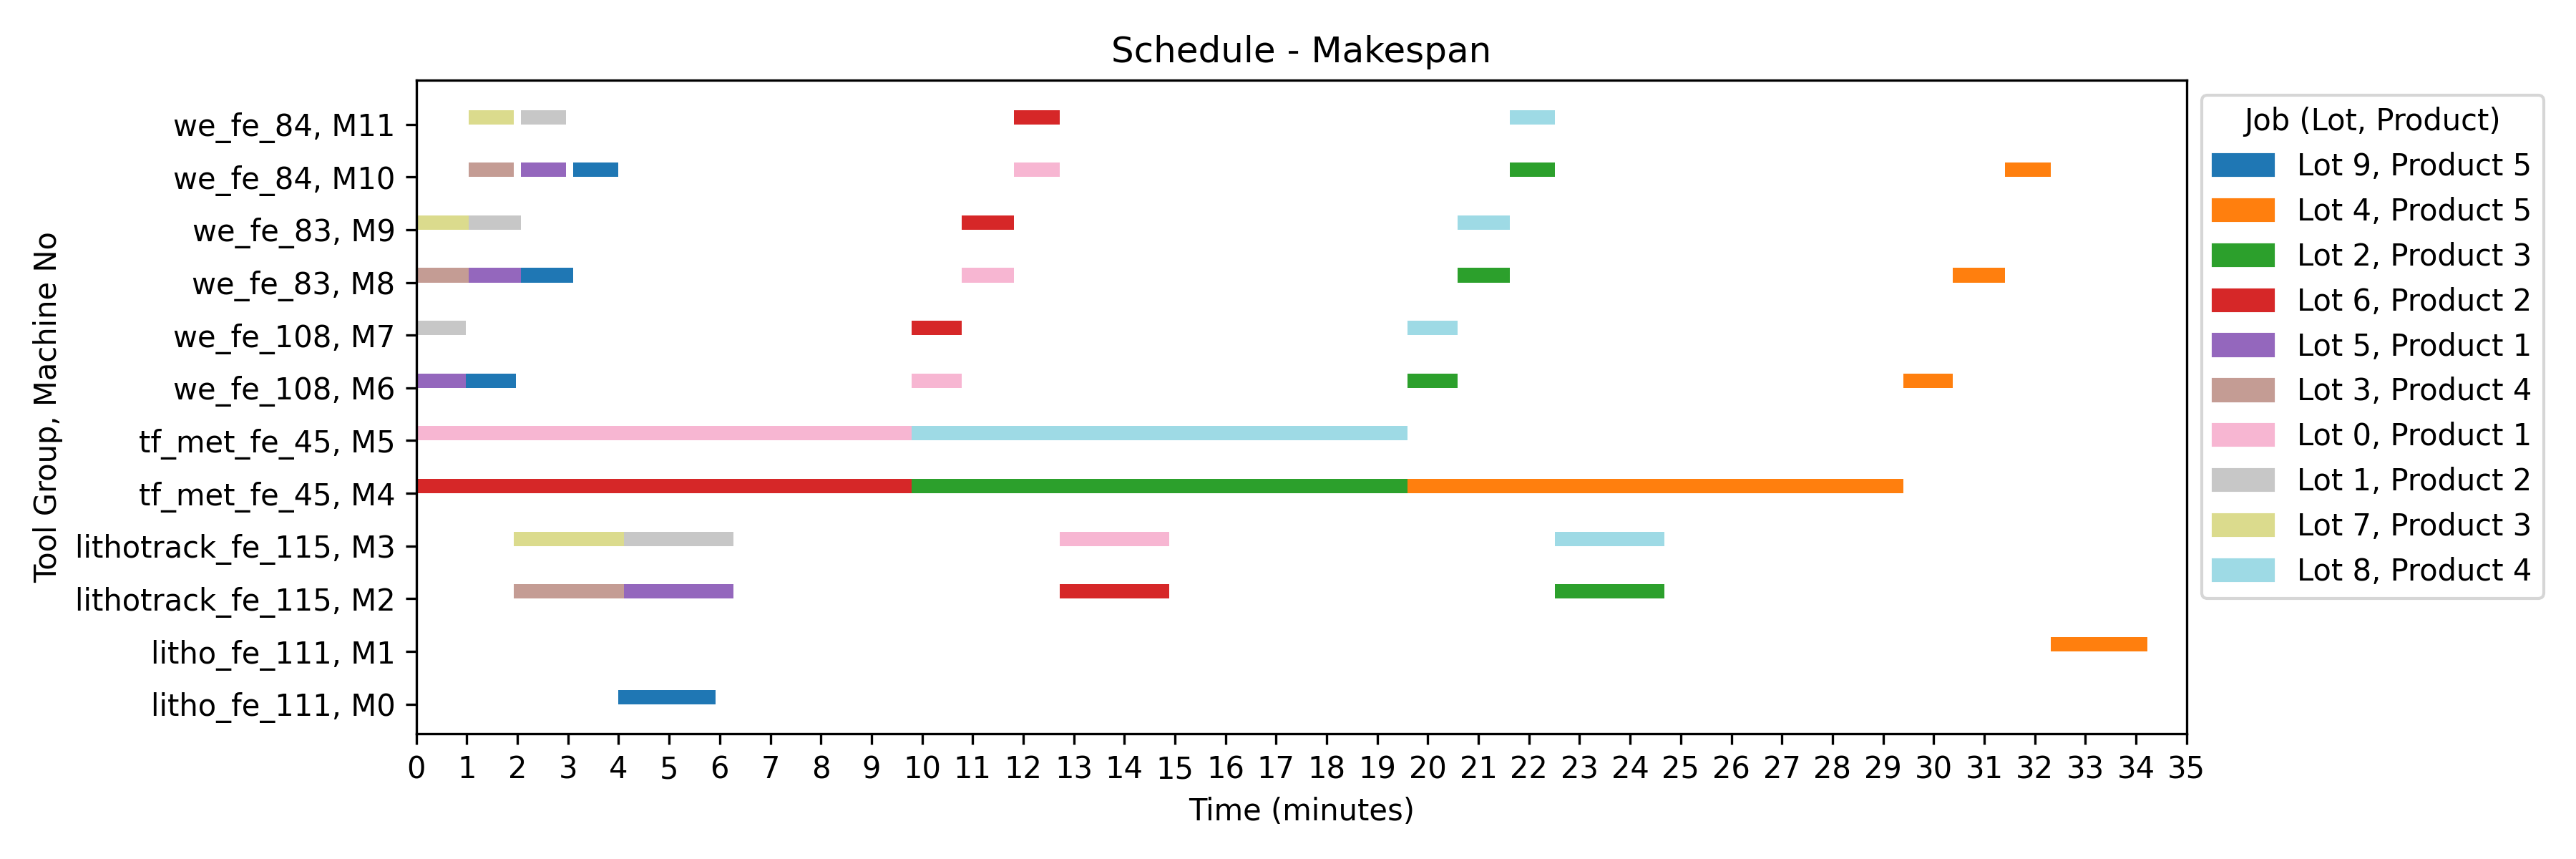
\includegraphics[width=\textwidth]{schedule_example_makespan.png}
	\caption{Feasible schedule for the instance in Table~\ref{tab:instance}}
	\label{fig:sch-makespan}
\end{figure}


To minimize the makespan, the algorithm selects a random edges and the selection process continues iteratively, with each step involving the evaluation of available operations that can be added to the existing sequence.
As operations gets selected, their corresponding edges are directed, indicating a fixed order. This directionality prevents the reselection of these operations. The procedure is completed once all operations are integrated into the sequence.
It is important to note that the chosen disjunctive edges connect operations based on their tool groups, meaning they do not dictate the machine assignments, which are determined in the subsequent phase. With a complete sequence of operations available, the second phase involves the allocation of each operation to the earliest available machine. This machine assignment step follows the order established in the first phase to create a feasible schedule that assigns machines and start and end times to all operations. The schedule is shown in Figure~\ref{fig:sch-makespan}.

\begin{figure}[ht]
	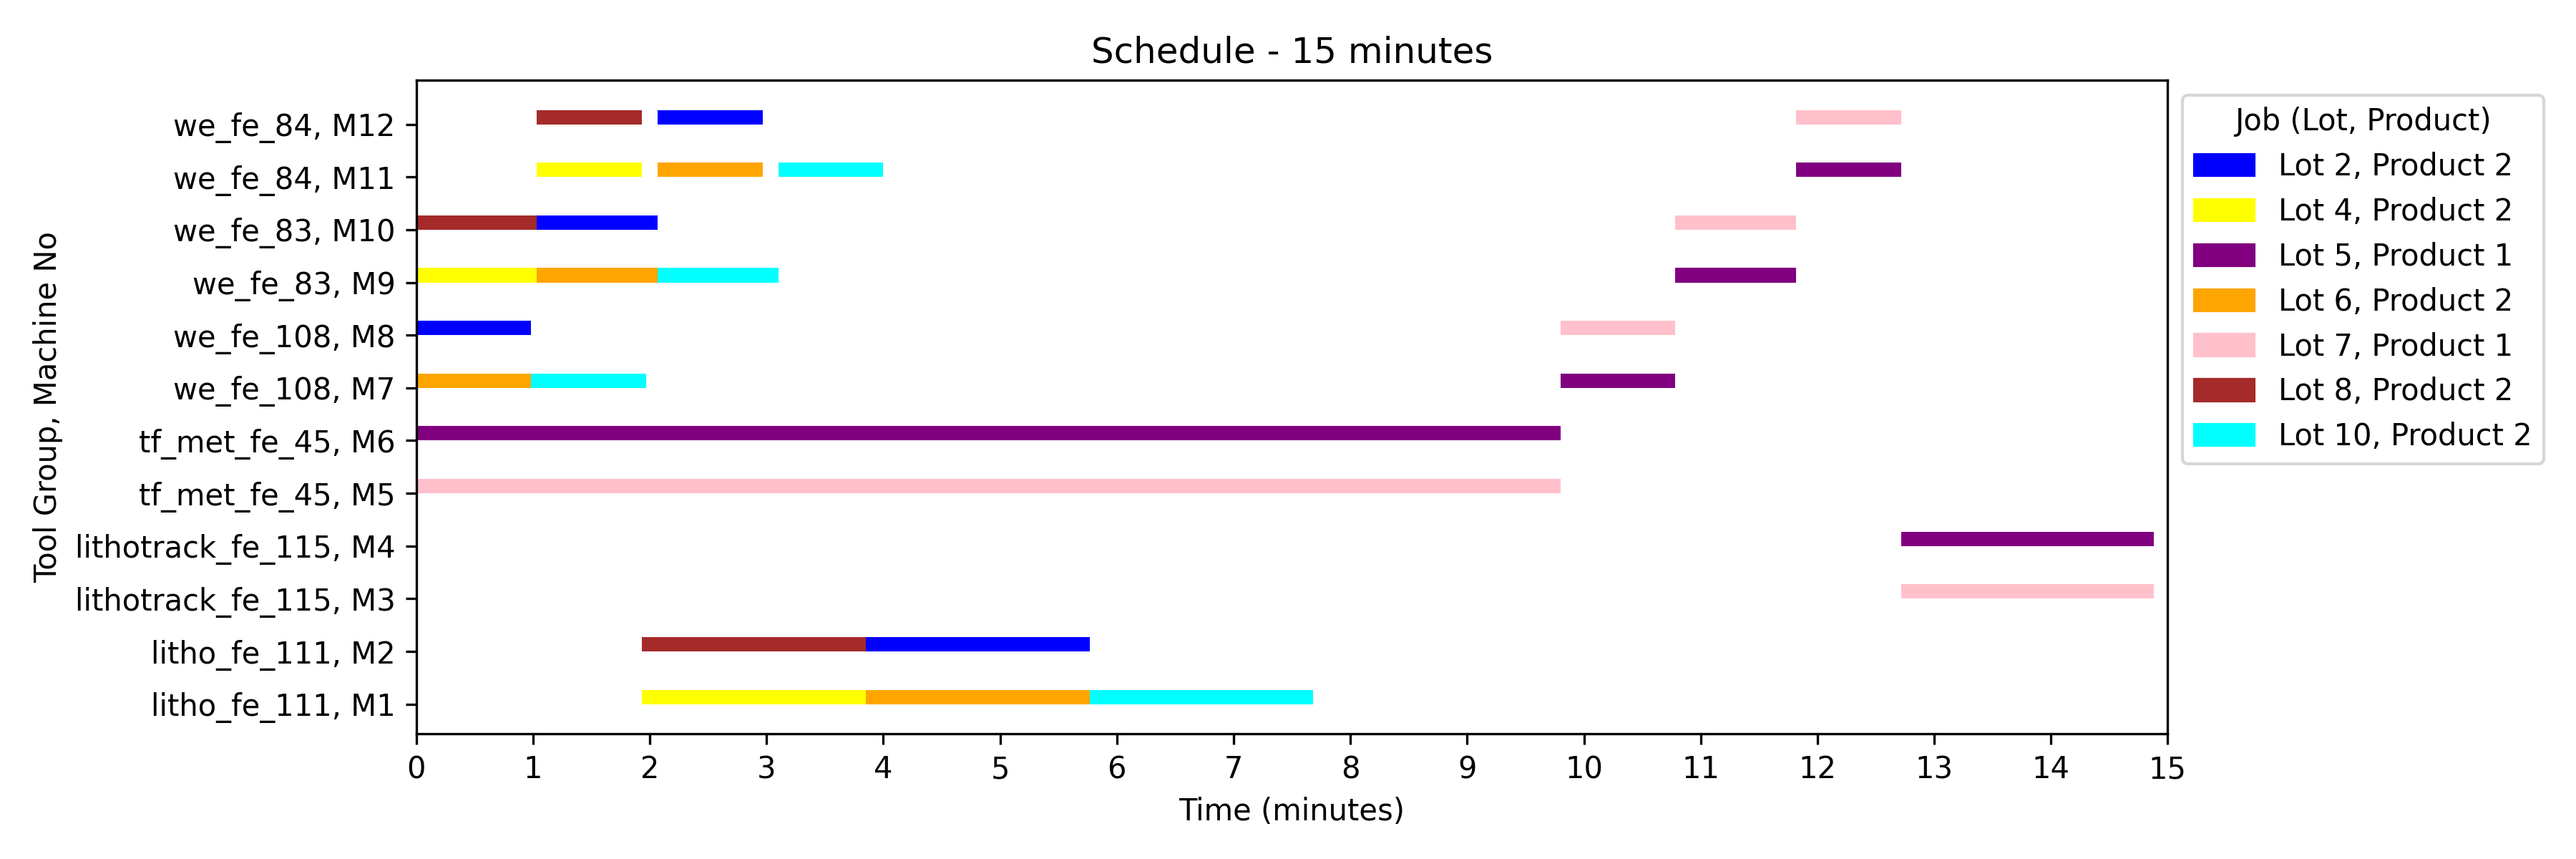
\includegraphics[width=\textwidth]{schedule_example_operations.png}
	\caption{Feasible schedule for the instance in Table~\ref{tab:instance}}
	\label{fig:sch-operations}
\end{figure}

To optimize operations within the planning horizon $h$, the algorithm initiates by selecting a random edge from the list of candidate operations. The start time for the first operations is set to zero. Based on the duration of each operation and taking into account the earliest available machine, the algorithm calculates the operation's end time. If this end time falls within the planning horizon $h$, indicating that the operation can be accommodated within the schedule, it is then added to the sequence. The algorithm continues this process iteratively, adding one operation at a time. In each iteration, it reassesses the remaining operations to determine which can fit into the updated schedule without exceeding the planning horizon. This iterative process persists until no more operations can be added within the designated periods, thereby optimizing the use of available time and resources within the planning horizon.
The schedule for 15 minutes is shown in Figure~\ref{fig:sch-operations}.

\subsection{Evaluation Module}
While each ant independently constructs a feasible schedule by means of the
GS procedure, the evaluation module collects the results obtained
by the ants in a GSACO-O iteration.
Among them, a schedule of shortest makespan or schedule of maximum operations is determined as outcome of the
iteration and stored as new best solution in case it improves over the schedules found in previous iterations (if any).
After evaporating pheromones~$\tau_e$ by $\rho\cdot\tau_e$,
where $\tau_z$ remains as minimum pheromone level if the obtained value
would be smaller,
the edges~$e$ that have been selected by the GS procedure for constructing the current best schedule receive a pheromone contribution and are updated to $\tau_e+c$.

Note that our contribution parameter $c$ is a constant,
while approaches in the literature often take the inverse of an objective value
\cite{turkyilmaz2020research}, i.e., of the makespan in our case.
The latter requires careful scaling to obtain non-marginal
pheromone contributions, in particular, when makespans get as large
as for SMSP instances.
We instead opt for pheromone contributions such that the
edges selected to construct best schedules are certain to have an increased chance
of getting re-selected in forthcoming iterations.

